\documentclass[12pt, letterpaper]{../assignment}
\usepackage{graphicx}
\usepackage{courier}
\usepackage{minted}
\usepackage{amsmath}
\usepackage{polynom}
\usepackage{commath}
\usepackage{amssymb}
\usepackage{amsfonts} 
\usepackage{color}
\usepackage{cancel}
\usepackage{enumitem}
\usepackage{graphicx}
\usepackage{multirow}
\usepackage{float}
\usepackage{bm}
\usepackage{tikz}
\usetikzlibrary{shapes,arrows}
\usepackage{booktabs}
\usetikzlibrary{patterns}

% Define Theme Colors
\definecolor{light-gray}{rgb}{0.2,0.2,0.2}
\definecolor{header-blue}{rgb}{0,0,0.7}
% \definecolor{header-blue}{rgb}{0.5137,0.8353,0.9176}
\definecolor{header-blue}{rgb}{0,0.8,0.95}
\definecolor{dark-gray}{rgb}{0.1,0.1,0.1}
\pagecolor{dark-gray}
\color{white}

\usemintedstyle{monokai}
\oddsidemargin = 0pt
\exercisesheet{Module 7}{Assignment}
\student{Austin Barrilleaux}
\university{\color{header-blue}Johns Hopkins University}
\school{\color{header-blue}Whiting School of Engineering}
\courselabel{EN 535.612}
\semester{Fall 2024}
\usepackage[backend=bibtex,style=numeric,sorting=none]{biblatex}
\bibliography{reference}

\definecolor{light-gray}{rgb}{0.2,0.2,0.2}
\setminted{bgcolor=light-gray,frame=lines,rulecolor=white}
\setlength{\parindent}{0pt}

\makeatletter
\patchcmd{\minted@colorbg}{\noindent}{\medskip\noindent}{}{}
\apptocmd{\endminted@colorbg}{\par\medskip}{}{}
\makeatother

\begin{document}

\subsection*{EXERCISE 7.1}
\subsubsection*{The slider descends along a curved guide as
the guide translates to the right at the constant speed $\bm{u}$.
The shape of the guide bar in terms of a body-fixed set of coordinates is $\bm{y = \beta x^2}$.
Generalized coordinates selected for this system are the fixed X and Y coordinates of the collar.
Independently derive the velocity and configuration constraint equations relating X and Y.
Then show that integration of the velocity constraint yields the configuration constraint.}

\begin{figure}[H]
    \centering
    \includegraphics[scale=0.9,frame]{images/Q7_1.png}
\end{figure}


Given the graphic provided, we can write that the velocities in the generalized coordinates are:

\begin{equation*}
\begin{aligned}
\dot{X} &= \dot{x} + u \\
\dot{Y} &= \dot{y} = 2 \beta x \dot{x}
\end{aligned}
\end{equation*}

The position of $X$ is defined as:

$$ X = ut + x \ \ \rightarrow \ \ x = X - ut $$

We can combine the above, and find that the velocity constraint for $\dot{Y}$ becomes:

$$ \dot{Y}  = 2 \beta \left( X - ut \right) \left( \dot{X} - u \right)  $$

This can be written as:

\begin{answer}
$$  2 \beta \left( X - ut \right)\dot{X}- \dot{Y} - 2 \beta \left( X - ut \right)u = 0  $$
\end{answer}

The configuration constraint is:

$$ Y = y = \beta x^2 = \beta \left( X - ut \right)^2 $$

More simply:

\begin{answer}
$$ Y =  \beta \left( X - ut \right)^2 $$
\end{answer}

Looking at the velocity constraint above, we know by reversing the chain rule for derivatives:

$$ \int f(g(x))\ g'(x)\ dx = F(g(x)) + C $$

Where for the velocity constraint:

\begin{equation*}
    \begin{aligned}
        f(g(x)) &= 2 \left( X - ut \right)\\
        g'(x) &= \left( \dot{X} - u \right)\\
        F(g(x)) &= \left( X - ut \right)^2
    \end{aligned}
\end{equation*}

Therefore:

$$ Y = \beta \int \left(2 \left( X - ut \right)\right) \left( \dot{X} - u \right) dt = 
\beta \int g(t)\ g'(t)\ dx = \beta \left( X - ut \right)^2  + C $$

We can integrate the velocity constraint to get the configuration constraint:

$$ Y =  \beta \left( X - ut \right)^2 + C $$

If the initial condition constant of integration, $C$ is zero:

\begin{answer}
    $$ Y =  \beta \left( X - ut \right)^2 $$
\end{answer}


\subsection*{EXERCISE 7.12}
\subsubsection*{The figure shows a disk that is constrained to roll
without slipping on a horizontal XY plane,
such that its plane remains vertical.
Let the position coordinates X and Y of the geometric center,
the heading angle $\bm{\Psi}$,
and the spin angle $\bm{\phi}$ be generalized coordinates.
Describe the velocity constraints between these generalized coordinates.
From those results, determine the number of degrees of freedom,
and whether the system is holonomic.}

\begin{figure}[H]
    \centering
    \includegraphics[scale=0.7,frame]{images/Q7_12.png}
\end{figure}

This system can be defined by the following sketch:

\begin{center}



    \tikzset{every picture/.style={line width=0.75pt}} %set default line width to 0.75pt        

    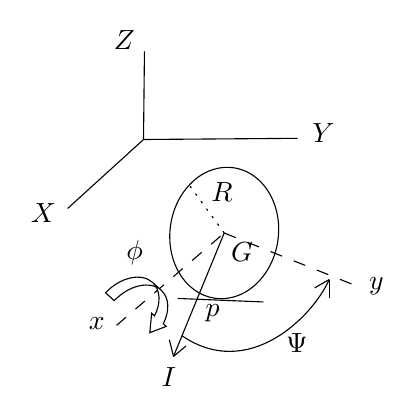
\begin{tikzpicture}[x=0.75pt,y=0.75pt,yscale=-1,xscale=1]
    %uncomment if require: \path (0,235); %set diagram left start at 0, and has height of 235
    
    %Shape: Ellipse [id:dp5700948325245387] 
    \draw   (161.55,116.98) .. controls (172.65,105.01) and (189.2,105.64) .. (198.52,118.38) .. controls (207.85,131.13) and (206.4,151.16) .. (195.3,163.13) .. controls (184.21,175.1) and (167.65,174.47) .. (158.33,161.73) .. controls (149.01,148.98) and (150.45,128.95) .. (161.55,116.98) -- cycle ;
    %Straight Lines [id:da6329481737698701] 
    \draw    (139.54,95.01) -- (140,52.5) ;
    %Straight Lines [id:da5628694482730268] 
    \draw    (103,128.23) -- (139.54,95.01) ;
    %Straight Lines [id:da2327292558887546] 
    \draw    (213.79,94.44) -- (139.54,95.01) ;
    %Straight Lines [id:da8344919129367174] 
    \draw  [dash pattern={on 4.5pt off 4.5pt}]  (126.57,184.54) -- (178.43,140.06) ;
    %Straight Lines [id:da5553400844068768] 
    \draw  [dash pattern={on 4.5pt off 4.5pt}]  (178.43,140.06) -- (242,165.5) ;
    %Straight Lines [id:da9747829335926719] 
    \draw    (156.04,171.59) -- (197.29,173.28) ;
    %Curve Right Arrow [id:dp3723246061248504] 
    \draw  [fill={rgb, 255:red, 255; green, 255; blue, 255 }  ,fill opacity=1 ] (148.06,167.64) .. controls (142.75,162.85) and (132.63,165.1) .. (125.45,172.65) -- (121.24,168.86) .. controls (128.42,161.3) and (138.55,159.06) .. (143.86,163.85) ;\draw  [fill={rgb, 255:red, 255; green, 255; blue, 255 }  ,fill opacity=1 ] (143.86,163.85) .. controls (147.8,167.41) and (147.98,173.84) .. (144.87,180) -- (143.47,178.74) -- (142.58,188.09) -- (150.48,185.06) -- (149.08,183.79) .. controls (152.19,177.63) and (152.01,171.2) .. (148.06,167.64)(143.86,163.85) -- (148.06,167.64) ;
    %Straight Lines [id:da6161249535946043] 
    \draw  [dash pattern={on 0.84pt off 2.51pt}]  (178.43,140.06) -- (161.55,116.98) ;
    %Straight Lines [id:da728985203136439] 
    \draw    (154,199.5) -- (178.43,140.06) ;
    %Straight Lines [id:da15944430387989095] 
    \draw    (160,194.5) -- (154,199.5) ;
    %Straight Lines [id:da9090041754305174] 
    \draw    (154,199.5) -- (152,191.5) ;
    %Curve Lines [id:da8450755379902992] 
    \draw    (158,189.5) .. controls (190,211.5) and (221,180.5) .. (229,162.5) ;
    %Straight Lines [id:da6193776594717113] 
    \draw    (222,166.5) -- (229,162.5) ;
    %Straight Lines [id:da5000963504738716] 
    \draw    (229,162.5) -- (229,171.5) ;
    
    % Text Node
    \draw (84,124.4) node [anchor=north west][inner sep=0.75pt]    {$X$};
    % Text Node
    \draw (124,41.4) node [anchor=north west][inner sep=0.75pt]    {$Z$};
    % Text Node
    \draw (219.66,86.28) node [anchor=north west][inner sep=0.75pt]    {$Y$};
    % Text Node
    \draw (168.21,173.18) node [anchor=north west][inner sep=0.75pt]    {$p$};
    % Text Node
    \draw (180.43,143.46) node [anchor=north west][inner sep=0.75pt]    {$G$};
    % Text Node
    \draw (130.05,142.14) node [anchor=north west][inner sep=0.75pt]    {$\phi $};
    % Text Node
    \draw (171,114.4) node [anchor=north west][inner sep=0.75pt]    {${\textstyle R}$};
    % Text Node
    \draw (112,179.4) node [anchor=north west][inner sep=0.75pt]    {$x$};
    % Text Node
    \draw (247,160.4) node [anchor=north west][inner sep=0.75pt]    {$y$};
    % Text Node
    \draw (147,203.4) node [anchor=north west][inner sep=0.75pt]    {$I$};
    % Text Node
    \draw (207,187.4) node [anchor=north west][inner sep=0.75pt]    {$\Psi $};
    
    
    \end{tikzpicture}
    
    
\end{center}

Constructing the angular velocity vector $\bar{\omega}$ of $xyz$ by vectorially adding the simple rotation rates according to:

$$ \bar{\omega} = \omega_1 \bar{e}_1 + \omega_2 \bar{e}_2$$

This gives us:

$$ \bar{\omega} = \phi \left(-\bar{i}\right) + \Psi \bar{k} = -\phi \bar{i}+ \Psi \bar{k}  $$

The velocity of the center of the disk at point $G$ from the no-slip point, point $p$ is defined as:

$$ \bar{v}_G^{xyz} = \cancelto{0}{\bar{v}_p} + \bar{\omega} \times \bar{r}_{G/p} $$

This evaluates to:


$$ \bar{v}_G^{xyz} = \bar{\omega} \times \bar{r}_{G/p}  = \left( -\phi \bar{i}+ \Psi \bar{k}  \right) \times R \bar{k} = R \dot{\phi}\ \bar{j}  $$

The rotation from the body frame to the (inertial) generalized coordinate frame is defined by the following sequence of rotations:

$$  R_\text{rot} = 
\left[\begin{array}{ccc} \cos\left(-\frac{\pi}{2} \right) & -\sin\left(-\frac{\pi}{2} \right) & 0\\ \sin\left(-\frac{\pi}{2} \right) & \cos\left(-\frac{\pi}{2} \right) & 0\\ 0 & 0 & 1 \end{array}\right]
\left[\begin{array}{ccc} \cos\left(\Psi \right) & -\sin\left(\Psi \right) & 0\\ \sin\left(\Psi \right) & \cos\left(\Psi \right) & 0\\ 0 & 0 & 1 \end{array}\right]$$


Or:

$$  R_\text{rot} = 
\left[\begin{array}{ccc} \sin\left(\Psi \right) & \cos\left(\Psi \right) & 0\\ -\cos\left(\Psi \right) & \sin\left(\Psi \right) & 0\\ 0 & 0 & 1 \end{array}\right] $$

Therefore, the velocity $\bar{v}_G$ can be expressed as:

$$ \bar{v}_G^{XYZ} = R_\text{rot}\ \bar{v}_G^{xyz} = 
\left[\begin{array}{ccc} \sin\left(\Psi \right) & \cos\left(\Psi \right) & 0\\ -\cos\left(\Psi \right) & \sin\left(\Psi \right) & 0\\ 0 & 0 & 1 \end{array}\right]
\left[\begin{array}{r} 0 \ \bar{i}\\ R \dot{\phi}\ \bar{j}\\ 0 \ \bar{k} \end{array}\right]
= \left[\begin{array}{r} R\ \dot{\phi} \,\cos\left(\Psi \right)\ \bar{I}\\ R\ \dot{\phi}\,\sin\left(\Psi \right)\ \bar{J}\\ 0\ \ \bar{K} \end{array}\right]$$

This can be expressed as the following velocity constraints:

\begin{answer}
$$ \dot{X} = R\ \dot{\phi}\,\cos\left(\Psi \right) $$
$$ \dot{Y} = R\ \dot{\phi}\,\sin\left(\Psi \right) $$
\end{answer}

Or: 

 $$ \dot{X} -R\ \dot{\phi}\,\cos\left(\Psi \right) = 0 $$
$$ \dot{Y} - R\ \dot{\phi}\,\sin\left(\Psi \right) = 0 $$

\begin{answer}
This system has $4$ generalized coordinates, $q_i = \left\{X, Y, \Psi, \phi\right\}$, and $2$ velocity constraints.
Subtracting the two gives us $2 \textbf{ degrees of freedom}.$
\end{answer}

To evaluate whether the system is holonomic,
we can isolate the coefficients of each generalized velocity:

$$ a_{11} = 1,\ a_{12} = 0,\ a_{13} = 0,\ a_{14} = -R\ \,\cos\left(\Psi\right), \ b_1 = 0 $$
$$ a_{21} = 0,\ a_{22} = 1,\ a_{23} = 0,\ a_{24} = -R\ \,\sin\left(\Psi\right), \ b_2 = 0 $$

Looking at the terms $a_{13}$ and $a_{14}$:

$$ \frac{\partial f_1}{\partial \Psi} = g_1\left(X, Y, \Psi , \phi\right)\ 0 = 0$$
$$ \frac{\partial f_1}{\partial \phi} = g_1\left(X, Y, \Psi , \phi\right) \left(-R\ \,\cos\left(\Psi\right) \dot{\phi}\right) $$

The second equation implies that the derivative of the function $f_1$ with respect to $\phi$, will contain $\Psi$, however the second implies that the derivative of the function with respect to $\Psi$ will be zero.
This is inconsistent. We see the same thing evaluating $a_{23}$ and $a_{24}$.
There is no integrating factor $g_1$ that can satisfy both of these, therefore the system is not integrable.

\begin{answer}
Since the velocity constraints are not integrable, the system is \textbf{non-holonomic}.
\end{answer}

% % \color{white}
% \hspace*{6em}\inputminted[frame=leftline,fontsize=\footnotesize]{matlab}
% {./matlab/Q6_8.m}
% % \color{black} 

% \begin{figure}[H]
%     \centering
%     \includegraphics[scale=0.7,frame]{images/Q5_13.png}
% \end{figure}




\end{document}

